%==========================================================================
% Exemplo de artigo para a Revista Brasileira de Computação Aplicada
%
% v0.5 versão atualizada em 02/09/2014 por Carlos Amaral Hölbig
% Rev1.: Modifado linha 17: \usepackage[latin1]{inputenc} para \usepackage[utf8]{inputenc} e linha de texto 120 de: $x$ para $\times\
% Copyright (C) 2014 Carlos Amaral Hölbig
% Programa de Pós-Graduação em Computação Aplicada
% Universidade de Passo Fundo
% Passo Fundo, Brasil
%==========================================================================

%==========================================================================
% Pacotes utilizados pela RBCA - não delete as linhas abaixo
%==========================================================================
\documentclass{RBCA}
\usepackage[T1]{fontenc}
\usepackage[utf8]{inputenc}%\usepackage[latin1]{inputenc}
\usepackage[brazilian]{babel}
\usepackage{graphicx}
%\usepackage{subfigure}
%\usepackage{epsfig}
\usepackage{hyperref}
\hypersetup{
  setpagesize  = false,
  colorlinks   = true,    % Colours links instead of ugly boxes
  urlcolor     = blue,    % Colour for external hyperlinks
  linkcolor    = black,   % Colour of internal links
  citecolor    = black    % Colour of citations
}
\urlstyle{same}
\usepackage{setspace}

\usepackage[num,bibjustif,recuo=0.8cm]{abntex2cite} 
% Referências e citações (em formato numérico, justificado e recuo de 0.8cm) utilizando o padrão ABNT
\citebrackets[] % coloca os números das citações entre [ ]

\usepackage{geometry}
\geometry{papersize={190mm,290mm},total={160mm,230mm}}
%==========================================================================

%==========================================================================
% Informações sobre a edição da revista: estes dados serão completados
% pelos editores da RBCA
%==========================================================================
\RBCAvolume{7}
\RBCAnumero{1}
\RBCApaginas{xx-xx}
\RBCAmes{abr}
\RBCAano{2015}
\setcounter{page}{1} % página inicial do artigo
%==========================================================================


%==========================================================================
% Dados do artigo: título, autores e filiação
%==========================================================================
\title{Revista RBCA: instruções para preparação de artigos}
\author
{
 Carlos Amaral Hölbig
   \footnote{Programa de Pós-Graduação em Computação Aplicada (PPGCA), UPF, Campus 1 - BR 285 - Passo Fundo (RS) - Brasil\\
   \texttt{\{holbig,carolina@upf.br\}}}
 \and
 Ana Carolina Bertoletti De Marchi
   \footnotemark[1]
   \and
Outro Autor
   \footnote{Endereço de Outro Autor\\
   \texttt{\{outroautor@email.br\}}\\ \\ \textbf{http://dx.doi.org/10.5335/rbca.2015.XXX}}
}
%==========================================================================


%==========================================================================
% Início do texto do artigo
%==========================================================================
\begin{document}

% \onehalfspacing

\maketitle
\thispagestyle{fancy}
\vspace{6pt}

\begin{abstract}
As instruções apresentadas neste texto objetivam auxiliar os autores na
preparação de artigos a serem submetidos para a Revista Brasileira de
Computação Aplicada (RBCA). Os artigos devem ser submetidos no modelo de
formato nas versões Word ou \LaTeX, disponíveis na página da revista. O resumo deve ser escrito
em Português e não deve ultrapassar 200 palavras, utilizando fonte do tipo Times,
tamanho 10, margens laterais reduzidas em 1 cm de cada lado, com duas linhas
em branco antes e depois do resumo. Os autores deverão colocar três palavras-chave
que destaquem os principais temas/áreas de pesquisa abordados no artigo. Caso o artigo seja escrito em língua inglesa a ordem do resumo/abstract deve ser invertida.
\end{abstract}

\begin{keywords}
Computação aplicada. Instruções. Revista RBCA. (em ordem alfabética)
\end{keywords}

\vspace{6pt}

\begin{abstractinenglish}
\emph{Resumo traduzido para a Língua Inglesa, em itálico, com a mesma formatação do resumo.}
\end{abstractinenglish}

\begin{keywordsenglish}
\emph{Applied computing. Instructions. Journal RBCA.} (Palavras-chave traduzidas para o inglês, em ordem alfabética)
\end{keywordsenglish}

\section{Instruções gerais}
A Revista Brasileira de Computação Aplicada (RBCA) é uma revista vinculada ao Programa de Pós-Graduação em Computação Aplicada (PPGCA) do Instituto de Ciências Exatas e Geociências da Universidade de Passo Fundo. A RBCA visa disponibilizar à comunidade científica artigos que apresentem uma perspectiva interdisciplinar da aplicação da Computação em diferentes áreas do conhecimento. Os artigos submetidos a RBCA deverão ter entre 10 a 15 páginas e serão publicados eletronicamente. Os idiomas aceitos pela revista são o português e o inglês. Alertamos aos autores para que a preparação do documento seja feita de forma cuidadosa, tanto em seu conteúdo técnico como em sua correção gramatical. Termos em inglês utilizados na área NÃO deverão estar em itálico.

\section{Seção}
O título de seção deve ser em negrito, numerado automaticamente (1, 1.1,..), Times 12, com 14 espaços antes e 12 após. Este espaçamento pode ser ligeiramente alterado quando houver necessidade de completar uma página. A primeira linha de cada parágrafo possui indentação de 1 cm e o espaçamento entre linhas deve ser simples. Cada parágrafo  deve ser separado do seguinte por 6 espaços. Este espaçamento pode ser ligeiramente alterado quando houver necessidade de completar uma página.

\subsection{Subseção}
Cada título de subseção deve ser em negrito, Times 10, com 12 espaços antes e 8 após. Este espaçamento pode ser ligeiramente alterado quando houver necessidade de completar uma página.

\subsection{Área de impressão}
A área de impressão é de 16cm $\times$ 23cm sendo o tamanho da página definido como 19cm $\times$ 29cm. A margem superior e a inferior deverão ter 3cm e as margens laterais 1,5cm. O texto deve ocupar a linha inteira e as figuras não podem ultrapassar as margens definidas. Procure preencher toda a área de impressão da página de modo a não deixar mais do que 2 cm em branco no final de cada página.

\subsection{Títulos}
Os títulos, incluindo o título principal, devem iniciar com letra maiúscula, sendo as demais letras minúsculas e todas as demais palavras do título devem iniciar por letra minúsculas. Por exemplo: "Revista RBCA: instruções para preparação de artigos".

\subsection{Rodapé e numeração de páginas}
O rodapé contém a identificação da revista, seu volume e número e a numeração de páginas e é alinhado à esquerda. A primeira página deve conter o cabeçalho.

\subsection{Legendas de tabelas e de figuras}
As tabelas devem ser numeradas a partir de 1 e referenciadas como "Tabela x". A legenda deverá estar no topo da tabela, conforme exemplo mostrado na Tabela~\ref{tab:exemplo}. Para as figuras proceda do mesmo modo com as tabelas.

\begin{table}[ht]
\begin{center}
\caption{Formatos de títulos}
\label{tab:exemplo}
\begin{tabular}{lll}
    \hline
	Item (alinhamento) & Exemplo & Font e estilo\\
	\hline
	Título (esquerdo) & \Large\textbf{Título do artigo} & 14~pontos, negrito\\
	Seção (esquerdo) & \large\textbf{1~Introdução} & 12~pontos,	negrito\\
	Subseção & \textbf{2.1~Área de impressão} & 10~pontos,	negrito\\
	Terceiro nível & \textbf{2.2.1~Testes} & 10~pontos,	negrito\\
	Quarto nível & \emph{2.2.1.1~Observação} & 10~pontos,	itálico\\
	$\cdots$ & $\cdots$ & $\cdots$\\
	\hline
\end{tabular}
\end{center}
\end{table}

\subsection{Códigos de programas}
Listagens de código de programas devem usar um outro estilo de fonte, por exemplo, Courier 10, para que recebam destaque.  As listagens não são consideradas figuras, de modo que não necessitam ter legenda. Para fins de referência, as linhas do código podem  ser numeradas. Por exemplo, o código a seguir mostra uma classe Java, onde a linha 6 inicia um comando que se estende por diversas linhas.

\begin{verbatim}
 1. import java.util.Random;
 2. class Aleatorios {
 3.   public static void main (String[] args) {
 4.     Random qq=new Random();
 5.     for (int k=1;k<10;k++)
 6.       System.out.println("Método nextInT() da classe Random: " +
 7.         qq.nextInt(100) + "\nUsando o método Math.random(): " +
 8.         Math.random());
 9.   }
10. }
\end{verbatim}

\subsection{Fórmulas e equações}
Equações e fórmulas devem ser colocadas em uma nova linha, centralizadas e numeradas consecutivamente para fins de referência,
como pode ser observado em (\ref{eq:exemplo}). As equações devem ser referências conforme linha anterior, citado apenas o número da equação entre parênteses.

\begin{equation}
x + y = z
\label{eq:exemplo}
\end{equation}

\subsection{Figuras e fotografias}
As figuras devem ser integradas ao texto, centralizadas de acordo com as margens. Para testar a visibilidade dos detalhes de suas figuras, por favor, faça a geração de um arquivo imagem de impressão (\emph{postscript}) e observe se todos os detalhes estão perfeitamente visíveis e os textos legíveis.  As figuras devem ser numeradas e todas devem ter uma legenda explicativa. Centralize a legenda entre as margens, use fonte Times 10, e mantenha uma distância de cerca de 6 pontos antes e após, conforme exemplo mostrado na Figura~\ref{fig:proc}.

Tenha especial cuidado com figuras feitas diretamente com as ferramentas Word. Permita que elas flutuem sobre o texto, sem âncoras. Se houver necessidade de inserir uma quebra de página antes da figura, certifique-se que a página anterior esteja completa. Se a figura ocupar uma página completa, certifique-se que esta não ultrapasse as margens. Evite colocar figuras e tabelas no formato paisagem.

\begin{figure}[ht]
\begin{center}
\caption{Exemplo de figura}
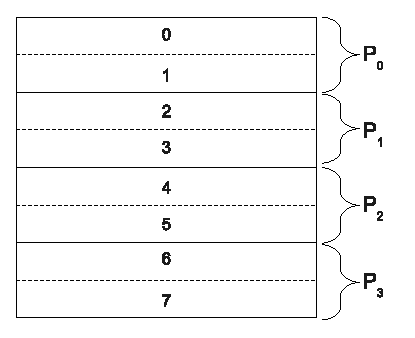
\includegraphics[scale=0.8]{figura.eps}
\label{fig:proc}
\end{center}
\end{figure}

\subsection{Notas de rodapé}
As notas de rodapé são usadas na primeira página para a identificação dos autores e, ao longo do texto, podem ser usadas para esclarecimentos.

\subsection{Submissão do artigo}
Ao submeter seu trabalho à Revista RBCA, verifique se você possui os seguintes arquivos, de acordo com o formato escolhido:

\begin{itemize} \setlength{\parskip}{0pt}% incluído pelo editor
\item \LaTeX: seus arquivos fonte (arquivo \textbf{.tex} para o texto, \textbf{.bib} para as referências bibliográficas e os arquivos das figuras) e arquivos ou macros adicionais que você tenha usado.
\item Word: seu arquivo fonte (arquivo  \textbf{.doc} ou \textbf{.docx}).
\end{itemize}

Para a submissão inicial do artigo, para iniciar o processo de avaliação, enviar pelo sistema da RBCA apenas o arquivo no formato PDF.

\subsection{Citações e referências}
A RBCA segue o formato de referências e citação da ABNT, em formato numérico, justificado e com recuo de $0.8 cm$. Para usuários de \LaTeX é utilizado do pacote \texttt{abntex2cite} (os pacotes constam no \emph{template} do modelo de artigo em \LaTeX). Ao longo do texto, as citações são feitas por meio de números consecutivos entre colchetes, de acordo com a ordem de citação. Ao final, a lista de referências deve ter o nome de Referências (negrito, fonte Times 12 e alinhado à esquerda), sem numeração de seção. Não colocar quebra de página antes. Nas referências que possuírem mais de três autores deverá ser colocado o nome do primeiro autor seguido de 'et al.'. As referências devem seguir a ordem de citação no texto e devem estar formatadas da seguinte forma: livro -- \cite{Dongarra:2003}; capítulo de livro -- \cite{holbig2004}; artigo em periódico -- \cite{holbig2013}; artigo em conferência internacional -- \cite{holbig2014} e \cite{holbig2011}; artigo em conferência nacional -- \cite{tibuski2013}; teses/dissertações -- \cite{holbig2005}; relatórios técnicos -- \cite{holbig03c} e outras produções -- \cite{Tierney2014}. Exemplos destas referências são apresentados na seção Referências.

\section*{Agradecimentos}
A seção Agradecimentos deverá ser colocada ao final do artigo, antes da seção Referências, sem numeração.

% não deletar as próximas três linhas - utilizadas para colocar a numeração da referência entre []
\makeatletter
\renewcommand\@biblabel[1]{{\parbox{0.8cm}{[#1]}}}
\makeatother

\bibliography{referencias} % arquivo referencias.bib que contém as referências bibliográficas utilizadas no artigo

\end{document} 